\documentclass[10pt]{beamer}

\usetheme[progressbar=frametitle]{metropolis}
\usepackage{appendixnumberbeamer}

\usepackage{booktabs}
\usepackage[scale=2]{ccicons}

\usepackage{pgfplots}
\usepgfplotslibrary{dateplot}
\usepackage{multicol}
\usepackage{lipsum}
\usepackage{graphicx}
\usepackage{xspace}
\usepackage{xcolor}
\usepackage{color}
\usepackage{animate}
\usepackage{listings}
\setbeamercolor{alerted text}{fg=red}

\definecolor{codegreen}{rgb}{0,0.6,0}
\definecolor{codegray}{rgb}{0.5,0.5,0.5}
\definecolor{codepurple}{rgb}{0.58,0,0.82}
\definecolor{backcolour}{rgb}{0.95,0.95,0.92}
\definecolor{codeone}{rgb}{0.51,0.55,0.27}

\lstset{
	frame=tb,
	language=C,
	breaklines = true,
	backgroundcolor=\color{backcolour},   
	commentstyle=\color{gray},
	keywordstyle= \color{codeone},
	%\color{magenta},
	numberstyle=\tiny\color{codegray},
	stringstyle=\color{codepurple},
	basicstyle=\footnotesize,
	breakatwhitespace=false,         
	breaklines=true,                 
	captionpos=b,                    
	keepspaces=true,                 
	numbers=left,                    
	numbersep=5pt,                  
	showspaces=false,                
	showstringspaces=false,
	showtabs=false,                  
	tabsize=2
}


\title{EEE212 Industrial Awareness and Group Project}
\subtitle{Smart Mini-Refrigrator}
\date{\today}
%\date{}
\author{Ali Khan, 1406769\\Lingxuan Kong, 1405867\\Rishabh Aggarwal, 1407014\\Shiyao Zhang, 1405896\\Yuhao Wang, 1405404\\Zuopeng Liu, 1406090}
\institute{Department of Electrical and Electronics Engineering, XJTLU}
% \titlegraphic{\hfill\includegraphics[height=1.5cm]{logo.pdf}}

\begin{document}
%\lstset{style=mystyle}
\maketitle
{
\begin{frame}{Table of contents}
  \setbeamertemplate{section in toc}[sections numbered]
  \tableofcontents[hideallsubsections]
\end{frame}
}
\section{Introduction}
{
\begin{frame}[fragile]{Smart Mini-refrigerator}
	T
\end{frame}
}


\section{Equipment used}
{	
	\begin{frame}(For the Mini-Fridge...)
	The following are the major components of the refrigerator
	\begin{enumerate}[<+- | alert@+>]
		\item Peltier Module and Cooler
		\item Arduino
		\item Relay
		\item Temperature Probe/Sensor
		\item Plexiglass
		\item Power Supply
		\item Foam Sheets
	\end{enumerate}
\end{frame}
}

{
	\begin{frame}{Peltier Effect}
		Peltier effect is the presence of heating or cooling at an electrified junction of two different conductors. \\
		\vspace{5mm}
		Current flow between the two conductors allows heat to be generated or removed from the junction.
	\end{frame}
}
{
	\begin{frame}
		\frametitle{Peltier Effect}
		\begin{figure}
			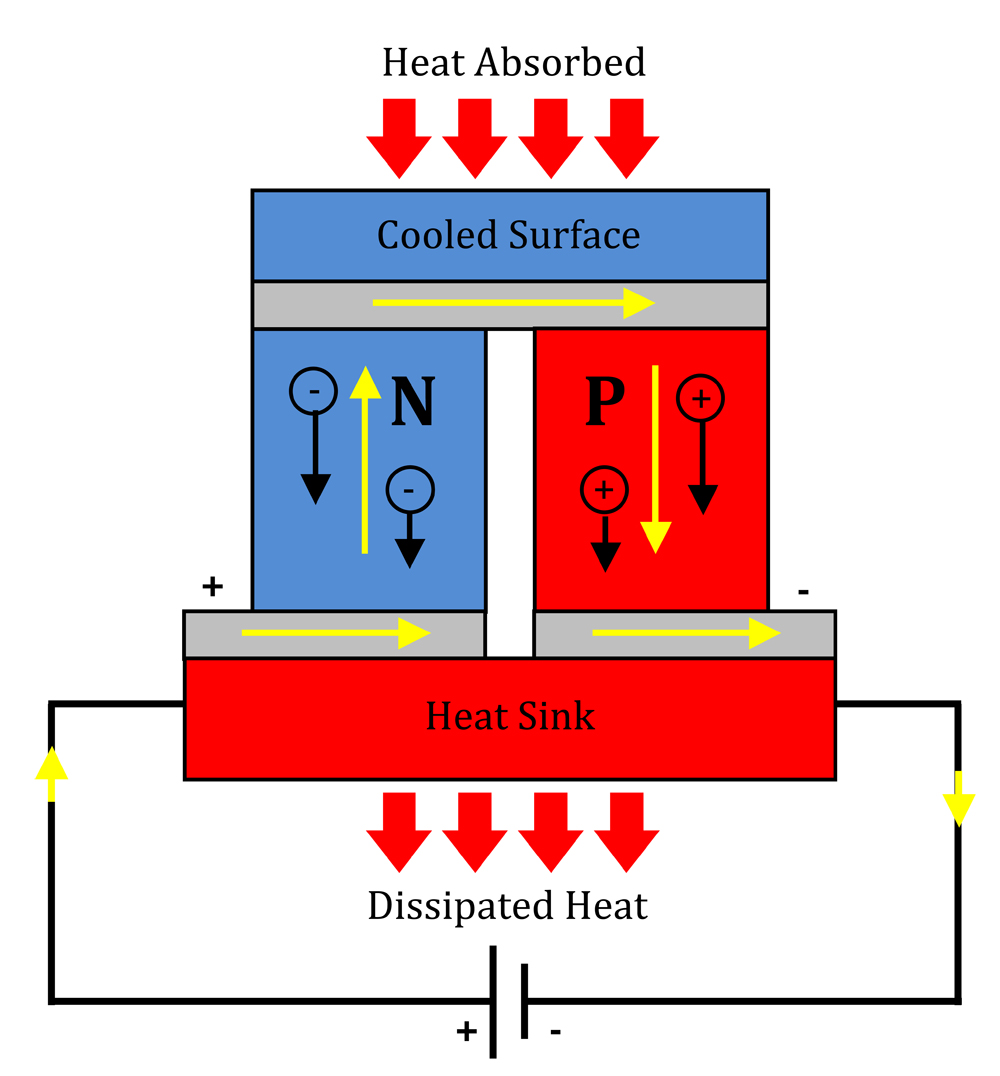
\includegraphics[scale=1.4]{images/peltier_effect}
			\caption{The Seebeck circuit as the peltier cooler}
		\end{figure}
	\end{frame}
}
{
\begin{frame}{Peltier Module}
	A Peltier Cooler is a solid state active heat pump, which transfers heat from one side of the device to the other. It consists a junction of two different type of materials\\
	\vspace{5mm}
	The flow of heat is dependent on the direction of current flow.
\end{frame}
}
{
	\begin{frame}
		\frametitle{Peltier Module}
		\begin{figure}[h!]
			\begin{minipage}[b]{0.4\linewidth}
				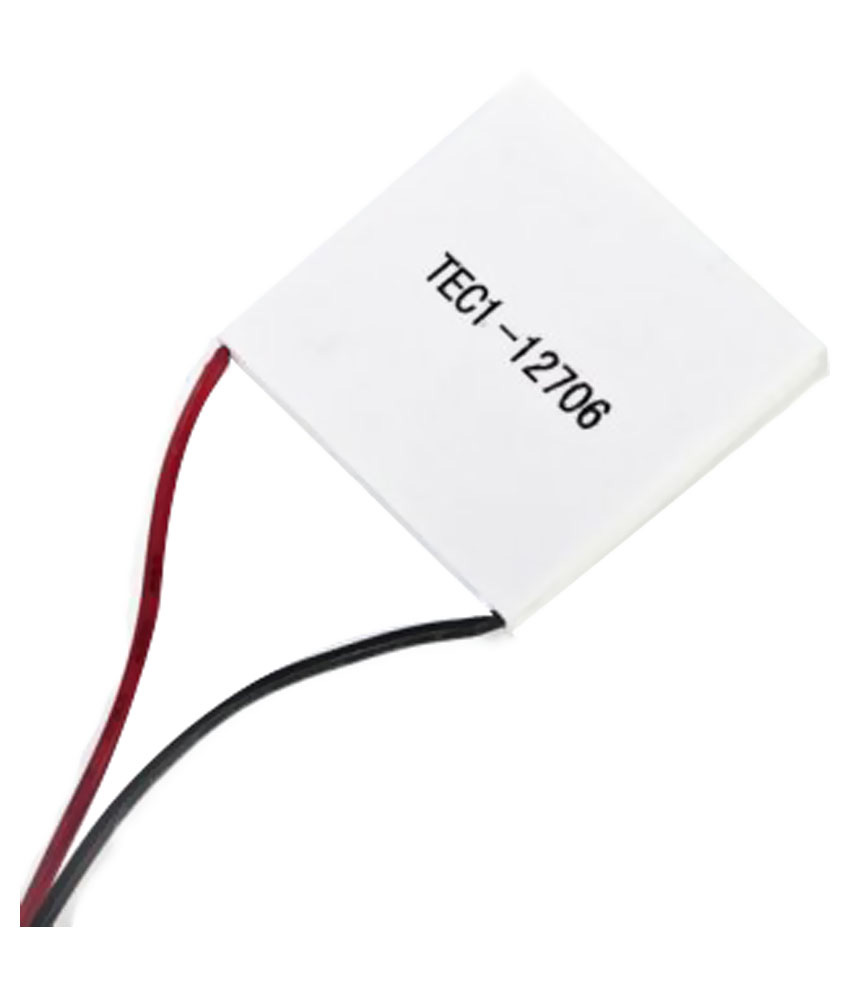
\includegraphics[width=0.8\linewidth]{images/peltier_module1}
				\caption{Peltier Module: TEC1-12706}
			\end{minipage}
			\begin{minipage}[b]{0.4\linewidth}
				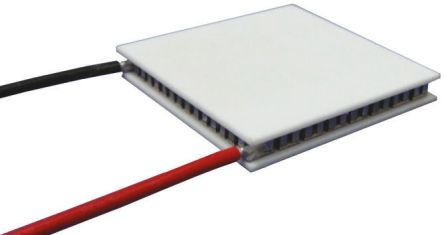
\includegraphics[width=0.8\linewidth]{images/peltier_module}
				\caption{Peltier Module Side view}
			\end{minipage}
		\end{figure}
	\end{frame}
}

{
	\begin{frame}
		\frametitle{Thermoelectric Cooler: How it works?}
		\begin{center}
			\animategraphics[autoplay,loop, width = 0.8\linewidth]{12}{images/peltcool/peltcool-}{0}{61}                          %,width=0.8\linewidth]{12                peltcool/pelt
		\end{center}

			
	\end{frame}
}
{
\begin{frame}{Thermoelectric Cooler Module we used}
	\begin{figure}[h!]
			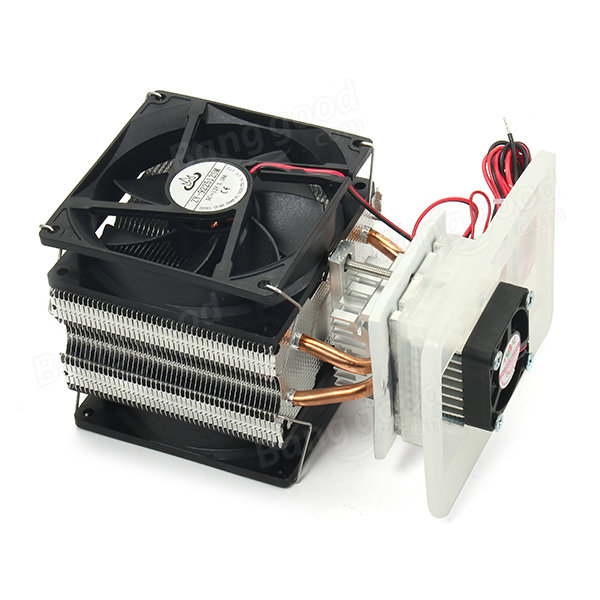
\includegraphics[scale=0.3]{images/thermo_cooler}
			\caption{12V 6A Thermoelectric Cooler Module}
	\end{figure}
\end{frame}
}

{
	\begin{frame}{Relay}
		A relay is an electrically operated switch. Many switch on/off mechanically using electromagnets.   \\
		\vspace{5mm}
		Relays are used where it is necessary to control a circuit by a specific low-power signal. For our project, we used a Magnetic Latching Relay with a single coil. The relay operates in one direction when power is applied with one polarity, and will reset when polarity is reversed. 
	\end{frame}
}
{
	\begin{frame}[!h]
		\frametitle{Magnetic Latching Relay}
		\begin{figure}
			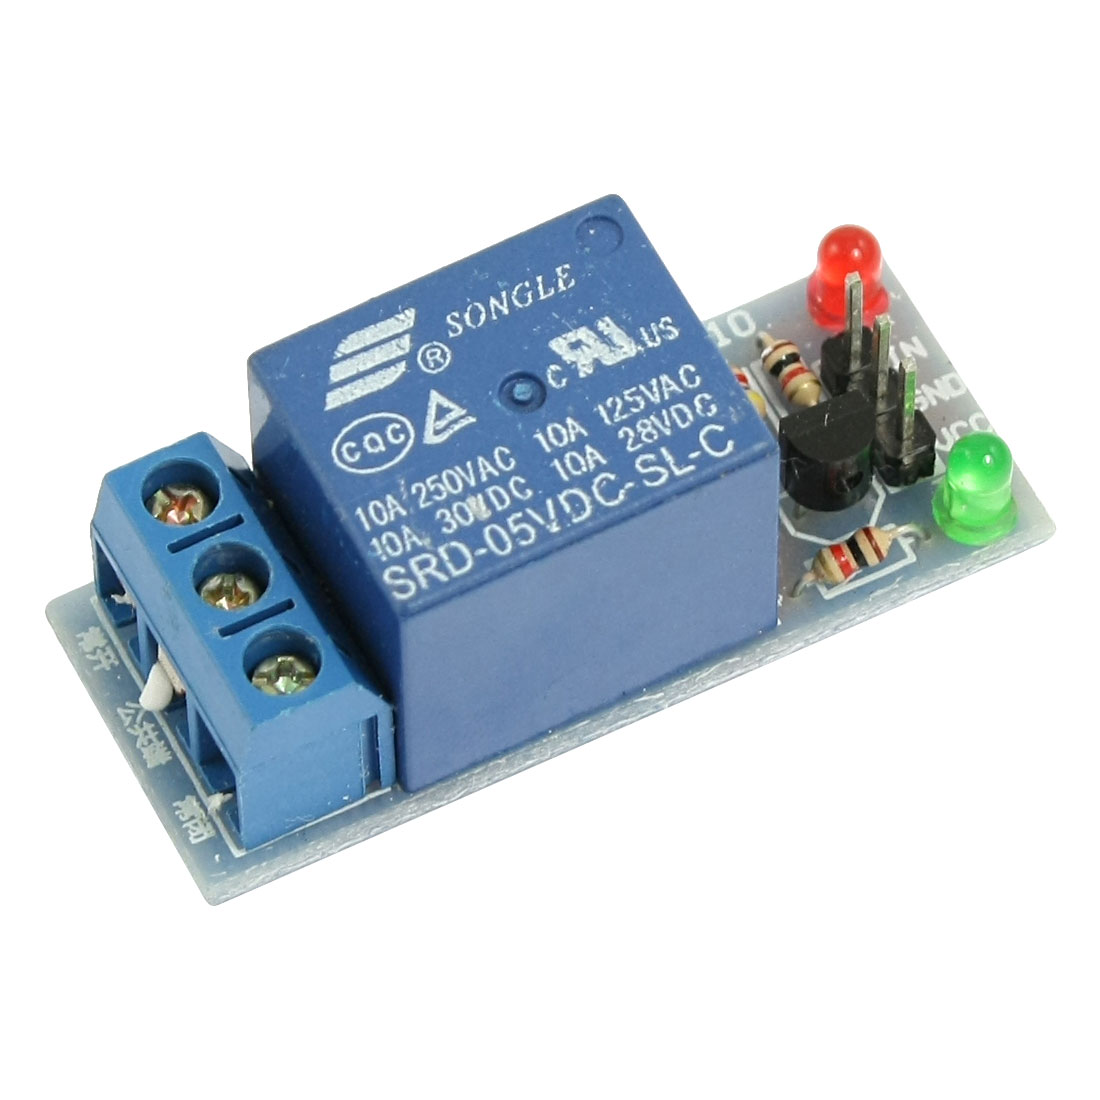
\includegraphics[scale=0.15]{images/relay}
			\caption{Single Coil Magnetic Latching Relay}
		\end{figure}
	\end{frame}
{
	\begin{frame}
		\frametitle{Temperature Sensor}
		\begin{figure}[h!]
			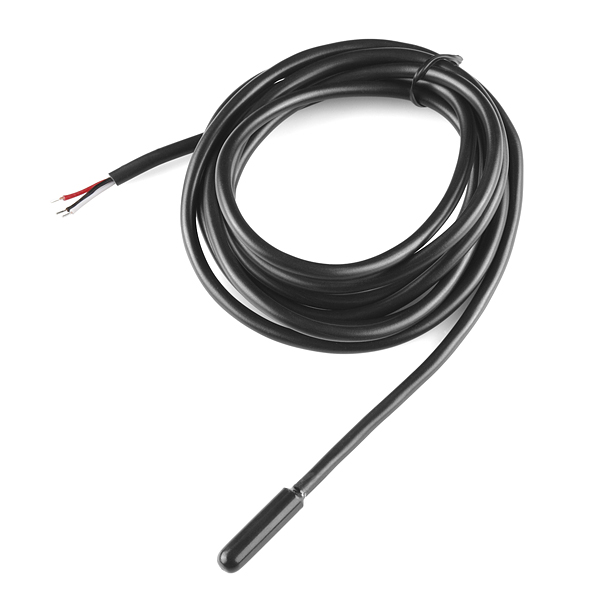
\includegraphics[scale=1]{images/sensor}
			\caption{DS18B20 Temperature sensor}
		\end{figure}
	\end{frame}
}
{
	\begin{frame}
		\frametitle{Arduino Micro-controller}
		\begin{figure}[h!]
				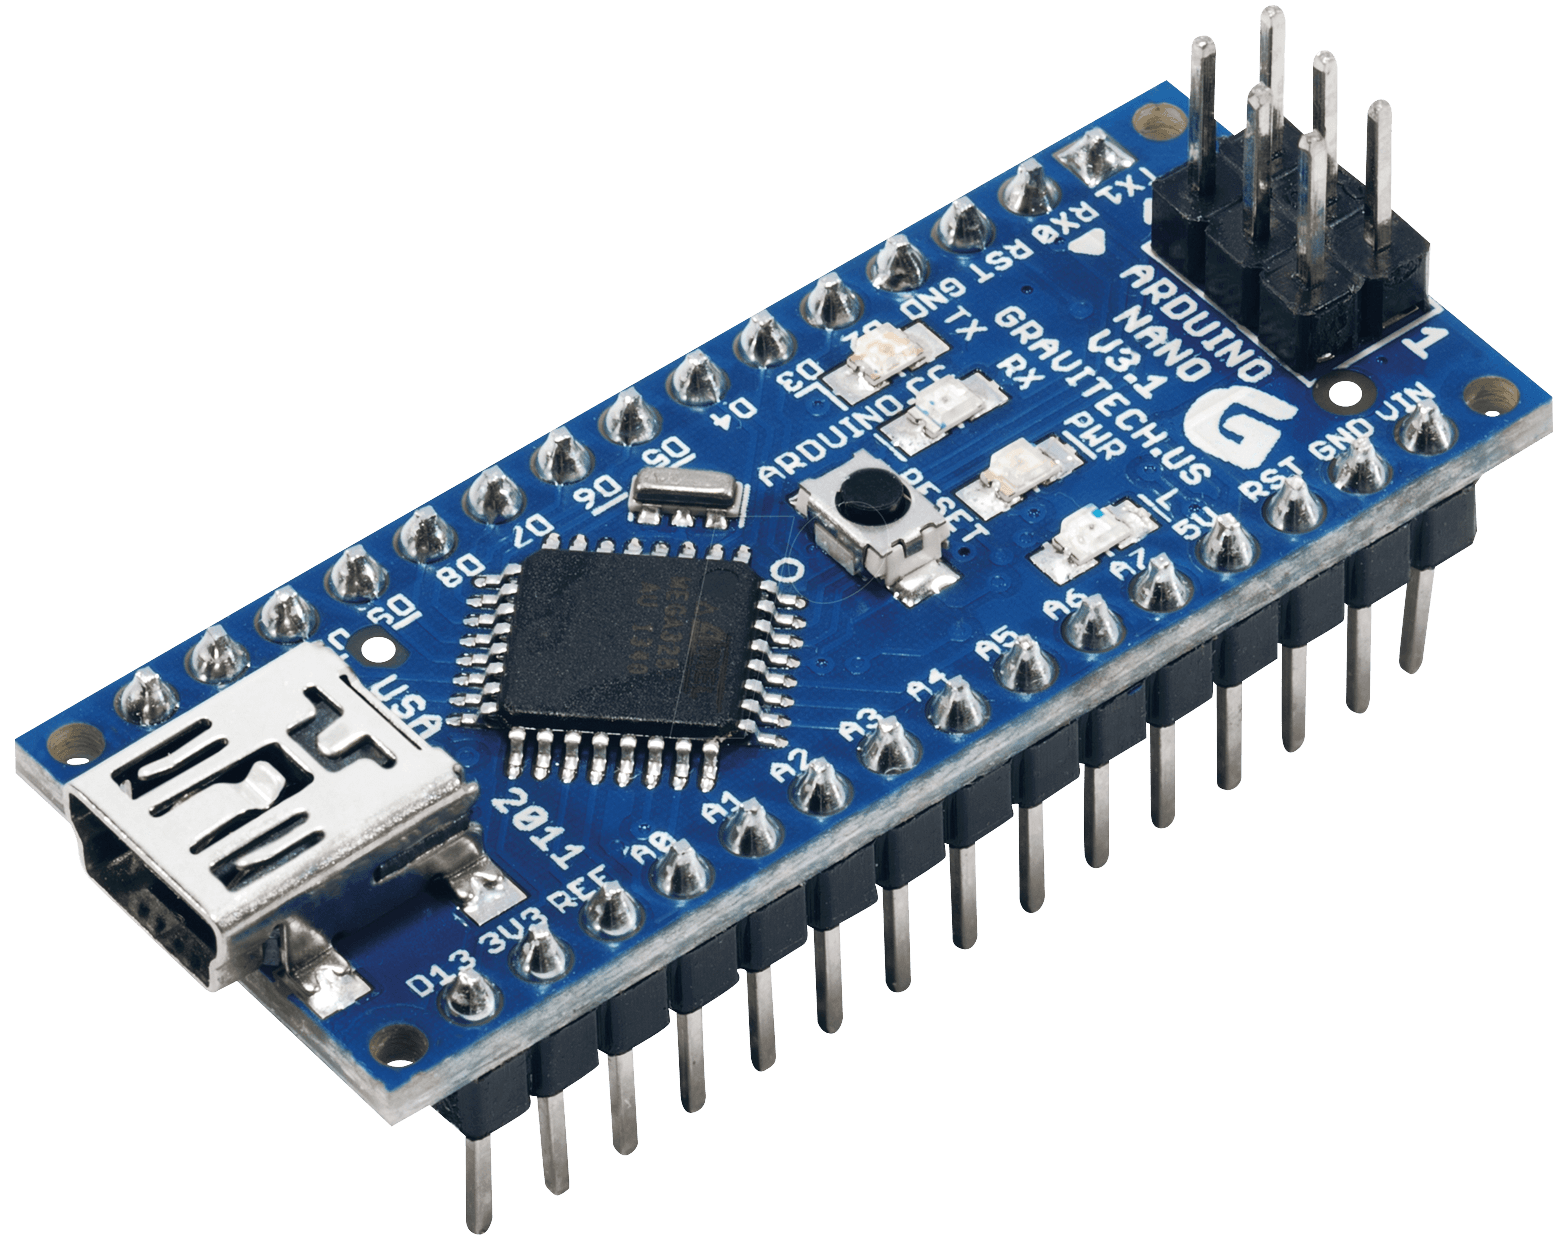
\includegraphics[scale=0.1]{images/arduino_nano}
				\caption{Arduino Nano Atmega328}
		\end{figure}
	\end{frame}
}

\section{Methodology}
{
	\begin{frame}{Circuit Schematic}
		\begin{figure}
			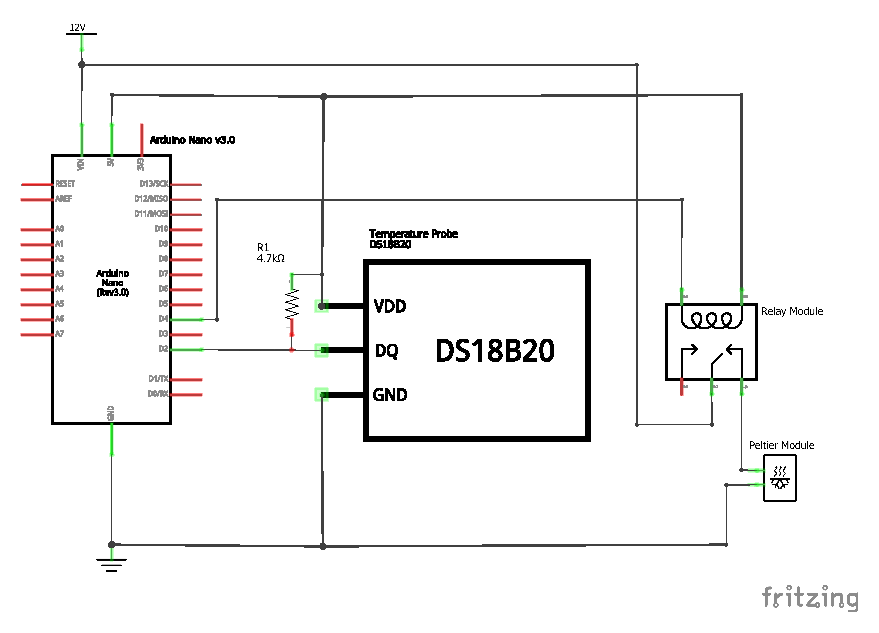
\includegraphics[scale=0.6]{images/mini_fridge_schem}
			\caption{Circuit Schematic of our control circuit}
		\end{figure}
	\end{frame}
}
{
	\begin{frame}{Arduino Code}
		\lstinputlisting[language = C++, lastline = 17]{code/F1VTS29IVO5D4XS/F1VTS29IVO5D4XS.ino}
	\end{frame}
}
{
	\begin{frame}{Arduino Code}
		\lstinputlisting[language = C++, firstline = 20]{code/F1VTS29IVO5D4XS/F1VTS29IVO5D4XS.ino}
	
	\end{frame}
}

{
	\begin{frame}{Procedure}
		The following steps give a picture of the procedure we followed when assembling our fridge:
		\begin{itemize}[<+- | alert@+>]
			\item The plexiglass panels were assembled into a box using hot glue
			\item Each panel was covered with foam board for insulation, inside and outside
			\item The thermoelectric cooler was installed
			\item Arduino circuit and power supply were installed 
			\item In the end, doors were fitted, back and front
		\end{itemize}
	\end{frame}
}

\section{Testing and Results}
{
	\begin{frame}{How we tested our product!}
		\begin{center}
			\begin{alertblock}{
					\bfseries{Temperature results and cooling duration\\}}
			\end{alertblock}
		\end{center}
	\end{frame}
}

\section{Strengths and Weakness}
{
	\begin{frame}{Strengths}
		\begin{itemize}[<+- | alert@+>]
			\item Powerful Peltier Module Cooler and power supply
			\item Cooling temperature is good
			\item Large Volume
			\item It is smart!. No manual temperature control needed
			\item 
		\end{itemize}
	\end{frame}
}
{
	\begin{frame}{Weaknesses}
		\begin{itemize}[<+- | alert@+>]
			\item Peltier Module cooler efficiency is low
			\item Improper Insulation
			\item Non-Portable
			\item Temperature Sensor sampling rate is small
			\item Overall fridge is a little fragile
		\end{itemize}
	\end{frame}
}
\section{Problems we faced!!}
{
	\begin{frame}{Problems we faced while doing our project}
		\begin{itemize}
			\item Choosing an appropriate Peltier Module and Power Supply
			\item Deciding the Volume of the fridge
			\item Choosing a good insulating material
			\item Choosing minimum and maximum temperature values for smart control
		\end{itemize}
	\end{frame}
}
\section{Improvements}
{
	\begin{frame}{What could we improve?}
		\begin{itemize}[<+- | alert@+>]
			\item Better insulate the fridge
			\item Use a more efficient thermoelectric cooler
			\item Use a sensor with fast sampling rate
			\item Have LED lighting inside the fridge
		\end{itemize}
	\end{frame}
}

\section{Conclusion}
{
		\begin{frame}{Conclusion}
	\begin{itemize}[<+- | alert@+>]
		\item The refrigerator is a combination product of hardware and software
		\item Cooperation: Every member is assigned with tasks
		\item The performance is satisfactory
	\end{itemize}
\end{frame}

}

\begin{frame}
\begin{center}
	\Huge Q \& A
\end{center}

\end{frame}


\end{document}
